\subsubsection{AMS1117}

El módulo \texttt{AMS1117} es un regulador de voltaje de 5V, el cual se utiliza para alimentar el microcontrolador. Es un regulador lineal de bajo \textit{drop-out} utilizado para suavizar la alimentación del microcontrolador. 

En su hoja de características indica que (en nuestra versión) tiene una tensión de salida fija de $5 V$, un \textit{dropout} mínimo de $1.3 V$ en el peor caso, una regulación de línea de hasta $10 mV$ para nuestra tensión de entrada y salida diseñadas, regulación de carga de hasta $35 mV$ y una corriente máxima de $0.9 A$ \cite{advancedmonolithicsystemsAMS1117}.

Utilizaremos el regulador a la salida del regulador reductor, con la finalidad de suavizar los picos de tensión que aparecen por la naturaleza conmutada de dicho regulador.

\begin{figure}[h]
    \centering
    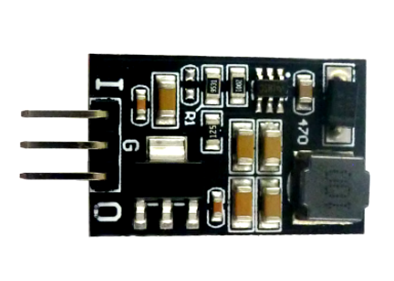
\includegraphics[width=0.5\textwidth]{images/2-hardware/componentes/AMS1117.png}
    \caption{\texttt{LDO AMS1117}}
    \label{fig:hardware/modulos/ldo-ams1117}
\end{figure}

\todo[inline,inlinewidth=0.9\textwidth]{Incluir imagen de los picos}